\documentclass[a4paper, 12pt]{article}

\usepackage[T1]{fontenc}

\usepackage{lipsum}
\usepackage{pifont}
\usepackage{amssymb}

\usepackage[utf8]{inputenc}
\usepackage[italian]{babel}
\usepackage{graphicx}
\graphicspath{ {./images/} }
\usepackage{spverbatim}
\usepackage{float}
\usepackage{url}
\usepackage{hyperref}

\usepackage{xcolor}
\definecolor{linkcolor}{RGB}{1,1,87}
\hypersetup{
    colorlinks,
    citecolor=black,
    filecolor=black,
    linkcolor=linkcolor,
    urlcolor=blue
}

\usepackage{xstring}



\newcommand{\code}[1]{\texttt{\StrSubstitute{#1}{_}{\_}}}
\newcommand{\Null}[0]{\code{NULL}}
\newcommand{\nota}[1]{\textbf{Nota}: #1}
\newcommand{\tbs}[0]{\textbackslash}




\newcommand{\makesub}[1]{%
  \saveexpandmode\noexpandarg
  \StrSubstitute{#1}{\_}{_}[\temp]%
  \restoreexpandmode
}
\newcommand{\target}[1]{%
  \makesub{#1}%
  \hypertarget{\temp}{}%
}
\newcommand{\codeattach}[1]{%
  \makesub{#1}%
  \hyperlink{\temp}{\code{#1}}%
}

\newcommand{\attach}[1]{%
  \makesub{#1}%
  \hyperlink{\temp}{\emph{#1}}%
}


\newcommand{\func}[1]{%
	\attach{#1}%
}

\setcounter{tocdepth}{4}
\setcounter{secnumdepth}{4}


\begin{document}\sloppy
  
\title{
  \textbf{
    \emph{Relazione homework 2}
  }
}  
\author{Luca Mastrobattista\\ Matricola: 0292461}
\date{}
\maketitle

\tableofcontents
\newpage
\section{Traccia dell'homework}
\subsection{Testo}
Analizzare con Ghidra, utilizzando lo strumento
disassemblatore/decompilatore, il programma eseguibile
hw2.exe contenuto nell'archivio hw2.zip (password: "AMW21").
Determinare il codice di sblocco che rende funzionale il
programma e riassumere in un documento tutte le informazioni
acquisite, la metodologia adottata ed i passi logici deduttivi
utilizzati nel lavoro di analisi.
\subsection{Scadenza}
Due settimane dalla data di assegnazione del lavoro: 14/11/2021
\subsection{Consegna}
Documento in formato PDF inviato come allegato ad
un messaggio di posta elettronica all'indirizzo del docente
("$<$cognome$>$@uniroma2.it"), con subject:
"[AMW21] HW2: $<$matricola studente$>$"

\newpage
\section{Ambiente di lavoro}
Il file eseguibile è stato caricato su Ghidra istallato su un sistema operativo Linux. \\
L'ambiente controllato di utilizzo è un sistema operativo Windows 10 virtualizzato con il software \emph{VirtualBox}, in cui sono istallati gli strumenti di monitoraggio.


\newpage
\section{Metodologia}

\subsection{Informazioni note a priori}
Dalla traccia dell'\emph{homework} si deduce che l'eseguibile risulta \emph{bloccato} in qualche modo, e solo con un particolare codice si riesce a farlo funzionare correttamente.

\subsection{Finalizzazione dell'obiettivo}
L'analisi dell'applicazione ha come obiettivo quello di individuare il codice di sblocco.

\subsection{Ottenimento del codice macchina}
Codice macchina fornito dal professore.


\subsection{Osservazione del funzionamento}
L'applicazione, una volta avviata, crea una finestra con un \emph{countdown} impostato a 30 minuti per default, ma questo tempo è modificabile. Premendo sul pulsante \emph{Go}, il conto alla rovescia inizia. È presente una casella di testo in cui inserire il codice da trovare. 
\begin{figure}[H]
\centering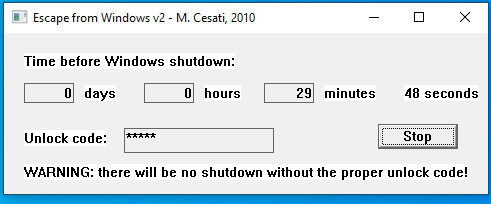
\includegraphics[scale=0.4]{lauch_of_program}
\end{figure}
Al termine del \emph{countdown}, se il codice inserito non è corretto, compare una finestra di avviso di codice errato:

\target{dialogo}
\begin{figure}[H]
\centering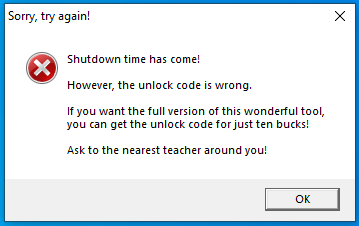
\includegraphics[scale=0.4]{error_code_ad}
\end{figure}

\subsection{Disassemblaggio del codice macchina}
Lo strumento che si è utilizzato è il software \emph{Ghidra}.

\subsubsection{Riepilogo risultati dell'import}
\begin{figure}[H]
\centering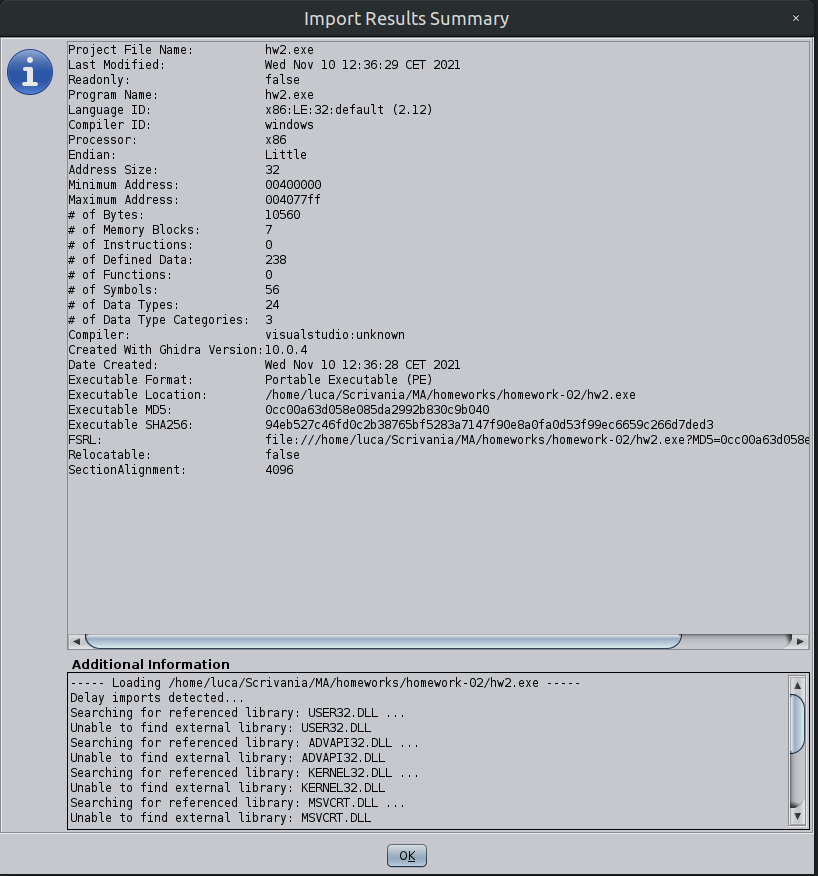
\includegraphics[width=\textwidth]{import_summary}
\end{figure}

\subsubsection{Informazioni aggiuntive}
\begin{spverbatim}
----- Loading /home/luca/Scrivania/MA/homeworks/homework-02/hw2.exe -----
Delay imports detected...
Searching for referenced library: USER32.DLL ...
Unable to find external library: USER32.DLL
Searching for referenced library: ADVAPI32.DLL ...
Unable to find external library: ADVAPI32.DLL
Searching for referenced library: KERNEL32.DLL ...
Unable to find external library: KERNEL32.DLL
Searching for referenced library: MSVCRT.DLL ...
Unable to find external library: MSVCRT.DLL
Searching for referenced library: GDI32.DLL ...
Unable to find external library: GDI32.DLL
Finished importing referenced libraries for: hw2b.exe
  [ADVAPI32.DLL] -> not found
  [GDI32.DLL] -> not found
  [KERNEL32.DLL] -> not found
  [MSVCRT.DLL] -> not found
  [USER32.DLL] -> not found

\end{spverbatim}

\newpage
\subsection{Ricerca del WinMain}
Cercando tra le varie librerie importate, in \code{USER32.DLL} ci sono le classiche \code{GetMessageA, TranslateMessage, DispatchMessageA}. Queste funzioni sappiamo essere le funzioni di gestione del \code{MainLoop}: cerchiamo allora le referenze a \code{GetMessage}. Questa funzione viene invocata solo una volta, nella funzione \codeattach{FUN_00401904_WinMain}, che quindi è il nostro \code{WinMain}.

\newpage
\section{Analisi}
\target{FUN_00401904_WinMain}
\subsection{FUN\_00401904\_WinMain}
Nella funzione, è interessante leggere come viene inizializzato il parametro di tipo \code{WNDCLASSEXA} e, in particolare, il campo \code{lpfnWndProc}. Infatti, questo campo sarà il puntatore alla \emph{window procedure} che eseguirà quando la finestra riceverà messaggi dal sistema operativo. Questo campo è settato all'indirizzo di \code{LAB_004012e0}, che quindi deve essere convertito in funzione. Questa sarà la funzione \codeattach{FUN_004012e0_window_proc}.

\target{FUN_004012e0_window_proc}
\subsection{FUN\_004012e0\_window\_proc}
Questa è la funzione che si occupa della gestione dei vari messaggi che arrivano all'applicazione. Ricordiamo che questa funzione non è invocata direttamente ma esegue all'occorrenza dei messaggi e, per questo motivo, il valore dei parametri dipende dal messaggio stesso che arriva.

\subsubsection{WM\_CREATE}
La gestione di questo messaggio è interessante. Per prima cosa viene recuperato l'\emph{handle} alla all'istanza dell'applicazione invocando \code{GetWindowLongA} con il secondo parametro impostato a \code{GWL_HINSTANCE}. In seguito, viene invocata una \code{SetWindowLongA}, con cui si impostano gli \emph{user data} associati con la finestra. Il valore passato è il valore puntato dal parametro di input \code{lParam}. Per messaggi di tipo \code{WM_CREATE}, il parametro \code{lParam} è un puntatore a struttura \code{CREATESTRUCT}. In questo caso si sta recuperando il primo valore della struttura, cioè \code{LPVOID lpCreateParams}. Se la finestra è stata creata con \code{CreateWindowEx}, questo campo contiene il valore del parametro \code{lpParam} passato alla funzione \code{CreateWindowEx}. La funzione \code{CreateWindowEx} viene invocata in \codeattach{WinMain} e, come parametro \code{lpParam}, prende il risultato di \codeattach{FUN_00401aab_init_ds}, cioè l'indirizzo della struttura dati di tipo \code{struct_appds_00406010} lì inizializzata. Capiamo che questa sia una struttura dati per come vengono settati alcuni parametri: prima si inizializza il valore dei 4 byte distanti 168 dall'indirizzo base all'\emph{handler} della finestra recuperata con la chiamata iniziale a \code{GetWindowLongA}, poi all'interno di un ciclo, partendo dall'indirizzo base, si aggiunge un offset che incrementa di un valore costante per assegnare dei valori.  In particolare, si inizializzano i bytes 172, 176, 180, 188, e 184 ai risultati di invocazioni di \code{CreateWindowExA}. Questo blocco di  codice termina invocando \codeattach{FUN_00401b74_show_time} e \codeattach{FUN_00401b20_create_timer}.\\
La struttura dati ha quindi il seguente aspetto:
\begin{figure}[H]
\centering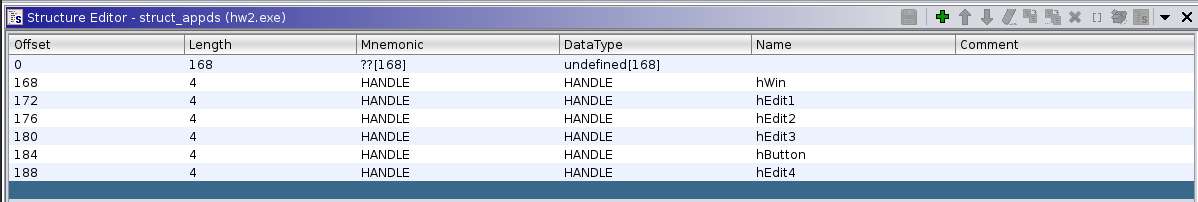
\includegraphics[width=\textwidth]{struct_after_wm_create}
\end{figure}

\target{FUN_00401aab_init_ds}
\paragraph{FUN\_00401aab\_init\_ds}
Questa funzione riceve in input un puntatore a funzione e inizializza una struttura dati definita alla variabile globale \code{struct_appds_00406010}. Qui vengono inizializzati altri campi della struttura: i primi quattro byte sono impostati a 0, i quattro byte in posizione 4 sono impostati a 1000, e quelli in posizione 12 sono impostati a 1800. Quest'ultimo ci ricorda il numero di secondi presenti in mezz'ora, che coincinde col valore di default dell'applicazione mostrato quando viene avviata e, per questo, è lecito pensare che sia il tempo in secondi dopo il quale l'applicazione dovrebbe venire spenta. In seguito ci sono due invocazioni della funzione \code{FUN_004023c0_invoke_snprintf}, funzione che non fa altro che invocare la funzione \code{_vsnprintf}. Quest'ultima funzione prende in input i seguenti parametri:
\begin{itemize}
\item un buffer in cui salvare la stringa formattata passata successivamente;
\item la dimensione massima, in byte, che possono essere salvati sul buffer;
\item una serie di parametri che servono a formattare la stringa da memorizzare.
\end{itemize}
La prima invocazione memorizza al massimo 128 caratteri sul buffer identificato nella struttura dati all'offset 24, impostandola alla stringa \code{"WARNING: there will be no shutdown without the proper unlock code!"}; la seconda, invece, memorizza al massimo 16 caratteri sul buffer identificato nella struttura all'offset 152, inizializzandolo alla stringa \code{" 0 seconds"}. Infine, si inizializzano i quattro byte in posizione 16 impostandoli a 0 e quelli in posizione 20 impostandoli al parametro ricevuto in input, di cui non conosciamo ancora il tipo.\\
La struttura dati ha adesso la seguente forma:
\begin{figure}[H]
\centering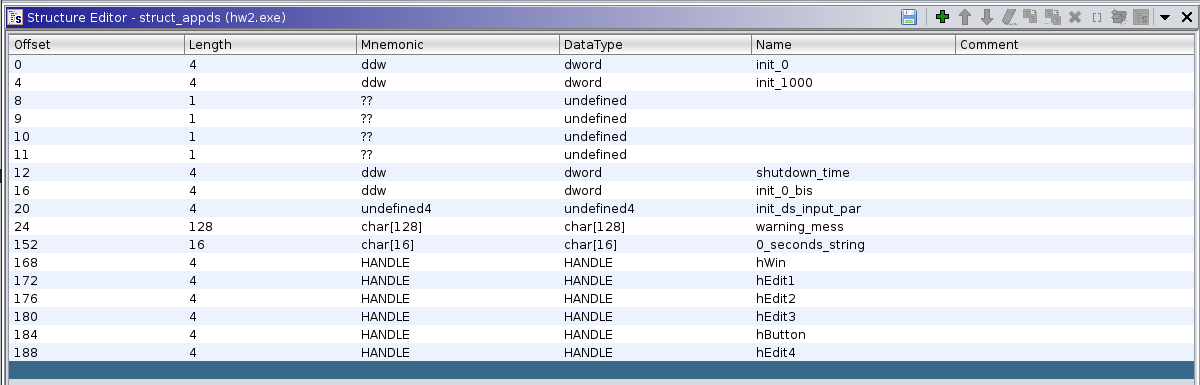
\includegraphics[width=\textwidth]{struct_after_wm_create_and_init}
\end{figure}

\target{FUN_00401b74_show_time}
\paragraph{FUN\_00401b74\_show\_time}
Questa funzione aggiorna il valore della stringa \code{0_seconds_string} della struttura dati, impostandola a:
\[
	s = (shutdown\_time - init\_0) - m \cdot 60
\]
dove m è calcolato come:
\[
	m = \frac{(shutdown\_time - init\_0) \cdot 1000}{init\_1000 \cdot 60}
\]
Il valore $m$ rappresenta il numero di minuti rimanenti, perché è risultato della divisione intera. Il valore s, invece, è il numero di secondi ancora rimanenti. Tutto ciò ha senso, però, solo se si assume che il campo \code{init_0} memorizzi in realtà il numero di secondi passati da quando è stato premuto il pulsante \emph{Go}; continuando su questa ipotesi, quel campo viene rinonimato in \code{elapsed_seconds}. \\
Successivamente, all'interno di un ciclo, viene calcolato il numero di giorni rimanenti, sottraendo a $m$ il valore 1440, cioè il numero di minuti in un giorno. Ad ogni iterazione, un contatore viene incrementato; il valore del contatore sarà impostato come valore della casella di testo relativa ai giorni. In seguito, utilizza lo stesso meccanismo per calcolare il numero di ore rimanenti, sottraendo questa volta il valore 60. Ciò che rimane, sarà il numero di minuti rimanenti. Vengono così aggiornati i valori delle caselle dei giorni, ore e minuti.

\paragraph{FUN\_00401b20\_create\_timer}
Questa funzione invoca semplicemente la funzione di libreria \code{SetTimer}, ma ci da molte informazioni riguardo ai parametri:
\begin{itemize}
\item il primo parametro è l'\emph{handle} alla finestra che deve essere associata con il timer;
\item il valore 0 come secondo parametro, per specificare la creazione del timer;
\item un valore intero, che specifica ogni quanto tempo eseguire un'operazione, in millisecondi. Il valore passato è il campo \code{init_1000}: ogni volta che trascorre un secondo verrà invocata una funzione;
\item un puntatore a funzione che viene invocata ogni volta che il tempo specificato nel parametro precedente passa. La funzione che viene impostata è \codeattach{FUN_00401c7b_timer_proc}.
\end{itemize}
Questa funzione restituisce un \code{UINT_PTR} che identifica il timer creato. Questo valore è inserito nella struttura dati, in corrispondenza del byte 8:
\begin{figure}[H]
\centering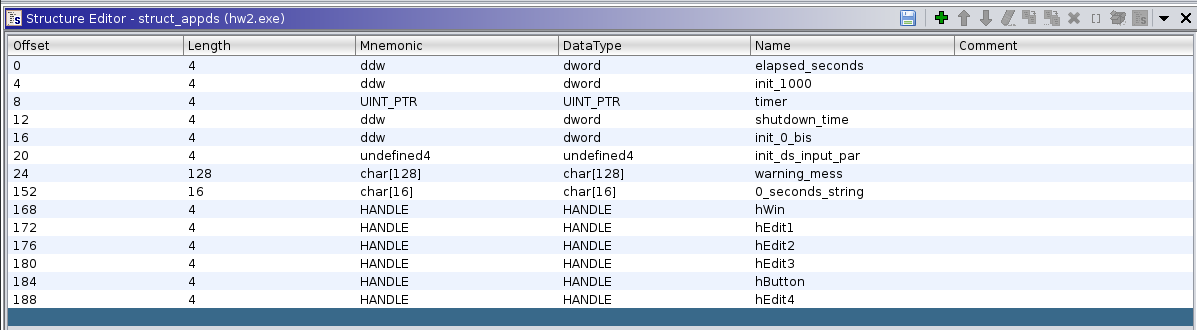
\includegraphics[width=\textwidth]{struct_after_wm_create_and_init_and_timer}
\end{figure}

Questa funzione, quindi, specifica le operazioni da fare ad ogni secondo trascorso. Potremmo quindi essere sulla strada giusta per la ricerca del codice. 

\target{FUN_00401c7b_timer_proc}
\paragraph{FUN\_00401c7b\_timer\_proc}
Questa funzione, per prima cosa, incrementa il campo \code{elapsed_seconds} della struttura dati \code{struct_appds}. Se è diverso da 0, aggiorna con la funzione \codeattach{FUN_00401b74_show_time} i valori mostrati. In seguito ridisegna la finestra. Con un controllo, si verifica se il campo \code{init_0_bis} è diverso da 0 e se \textbf{il tempo di shutdown è minore del valore di \code{elapsed_seconds} incrementato}: con quest'ultimo controllo, si sta verificando, in pratica, se il timer è scaduto. Se queste condizione sono entrambe vere, c'è un'istruzione di \code{CALL} che invoca il contenuto del campo in posizione 20 della struttura dati.
Capiamo quindi che quel campo della struttura è un puntatore a funzione:
\begin{figure}[H] 	
\centering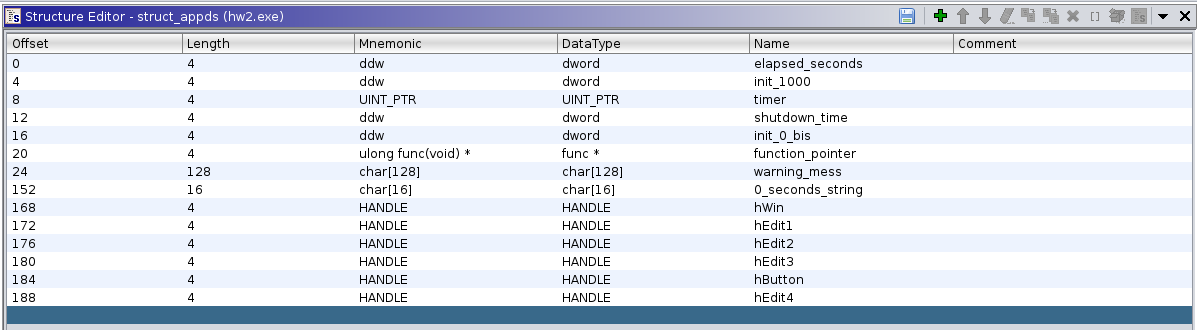
\includegraphics[width=\textwidth]{struct_func_pointer}
\end{figure}

È, con buone probabilità, la funzione che cerchiamo. Ritornando a \codeattach{FUN_00401aab_init_ds}, vediamo che il campo della struttura dati \code{function_pointer} viene inizializzato impostandolo al parametro di input. Questo parametro è l'indirizzo di \code{DAT_00403000}. Questa avrebbe quindi dovuto essere una funzione, tuttavia non è possibile convertirla. Disassemblando con Ghidra, cioè cliccando con il tasto destro sulle istruzioni e selezionando \emph{Disassemble}, si ottengono delle istruzioni macchina, anche se il flusso sembra essere corrotto. Questo può essere riparato cliccando col tasto destro sull'istruzione e premendo \emph{Clear Flow and Repair} come mostrato in \href{https://www.youtube.com/watch?v=H9DyLQ2iuyE}{questo video youtube}.\\
Una volta disassemblato e riparato il codice, si può analizzare la funzione invocata prima di terminare: \codeattach{FUN_00403000_check_on_exit}.

\target{FUN_00403000_check_on_exit}
\paragraph{FUN\_00403000\_check\_on\_exit}
Questa funzione viene invocata passandole come input la struttura dati \code{struct_appds_00406010}. Inizializza il campo \code{init_0_bis} a 0 e poi invoca la funzione \code{GetDlgItemTextA}. I parametri passati a questa funzione sono:
\begin{itemize}
\item il campo \code{hWin} della struttura dati, che memorizza l'\emph{handle} alla finestra;
\item il valore 5: questo rappresenta l'identificativo del \emph{control} da cui recuperare il testo. È l'identificativo della casella di testo che riceve il codice;
\item un buffer in cui memorizzare il testo recuperato. Il valore passato è l'area dello stack identificata da \code{ESP + 0x26}: il valore recuperato viene messo sullo stack;
\item il valore 30, che rappresenta la lunghezza massima recuperabile.
\end{itemize}
La funzione restituisce il numero di caratteri recuperati. \\

Il valore restituito viene confrontato col il numero 9 e, se è diverso viene invocata la funzione \codeattach{FUN_00401ff0_show_error_message} per poi ritornare. Se invece sono stati effettivamente letti 9 caratteri, si verifica che questi corrispondano a \code{3RnESt0!?}; il confronto è fatto byte per byte e, al primo errore, viene invocata la funzione \codeattach{FUN_00401ff0_show_error_message}. Se invece tutti i controlli passano, ci si prepara all'invocazione di una serie di funzioni: 
\begin{itemize}
\item \code{OpenProcessToken}, per aprire l'\emph{access token} associato al processo;
\item \code{LookupPrivilegeValueA}, per recuperare il \code{locally unique identifier (LUID)} usato sul sistema locale (identificato dalla stringa \code{NULL} passata come primo parametro);
\end{itemize}
Se queste invocazioni non falliscono, viene finalmente invocata \code{ExitWindowsEx}. \\

Si può quindi concludere l'analisi affermando che il codice che permette lo \emph{shutdown} è \textbf{3RnESt0!?}. \\

L'obiettivo dell'analisi è stato raggiunto in questo punto, e si potrebbe saltare alla fase di \attach{Verifica}; tuttavia non è stato ancora individuato il ruolo del campo \code{init_0_bis} della struttura dati e perciò, anche se non richiesto, viene riportato in seguito l'analisi delle funzioni che porta all'apprendimento del suo ruolo.

\target{FUN_00401ff0_show_error_message}
\paragraph{FUN\_00401ff0\_show\_error\_message}
Questa funzione invoca semplicemente una \code{MessageBoxA} per mostrare un dialogo con i seguenti parametri:
\begin{itemize}
\item \code{NULL}: l'handler all'\emph{owner window}. Avendo specificato \code{NULL}, la \emph{message box} non avrà una \emph{owner window};
\item la stringa \code{"Shutdown time has come!\tbs{}n\tbs{}nHowever, the unlock code is wrong.\tbs{}n\tbs{}nIf you want the full version of this wonderful tool,\tbs{}nyou can get the unlock code for just ten bucks!\tbs{}n\tbs{}nAsk to the nearest teacher around you!"}: rappresenta il messaggio da mostrare;
\item la stringa \code{"Sorry, try again!"}: rappresenta il titolo del dialogo creato;
\item il valore 16, che rappresenta \code{MB_ICONSTOP}: viene mostrata una icona col simbolo \emph{stop-sign}
\end{itemize}
La funzione termina invocando \code{PostQuitMessage}.\\
È effettivamente il \attach{dialogo} mostrato quando il codice è errato.





\subsubsection{WM\_DESTROY}
In questo blocco di codice si invoca la funzione \code{FUN_00401b54_kill_timer}, che a sua volta invoca la funzione di librearia \code{KillTimer} passando come parametro l'identificativo memorizzato nella \code{struct_appds_00406010} al campo \code{timer}. Il blocco di codice termina invocando \code{PostQuitMessage}.

\subsubsection{WM\_COMMAND}
Quando arriva un messaggio di questo tipo, il parametro \code{wParam} corrisponde all'identificativo del \emph{control} che genera il messaggio mentre \code{lParam} è l'\emph{handle} alla finestra di quel \emph{control}. In questo blocco di codice si controlla l'\emph{high word}, cioè la parola più significativa, per verificare che sia pari a 0 e si controlla che l'\emph{handle} contenuto in \code{lParam} passato in input alla funzione sia uguale a quella memorizzata nella struttura dati al campo \code{hButton}. Se le condizioni sono entrambe vere, si invoca \codeattach{FUN_00401dd6_button_clicked} prima di terminare.




\target{FUN_00401dd6_button_clicked}
\paragraph{FUN\_00401dd6\_button\_clicked}
Questa funzione controlla il campo \code{init_0_bis} per verificare se sia uguale a 0. In base al risultato del confronto, esegue 2 blocchi differenti prima di invocare una \code{RedrawWindow}.\\
Nel caso in cui \code{init_0_bis} sia 0, si cambia il testo mostrato nella finestra di indice 4, che corrisponde al pulsante: la scritta viene impostata a \code{"Stop"}. Dopodiché, si aggiorna il valore del campo \code{init_0_bis} e lo si imposta a 1 prima di invocare 4 volte la funzione \code{SendDlgItemMessageA}, una per ogni casella di testo. Il parametro \code{Msg} di queste invocazioni è 270, che corrisponde a \code{EM_SETREADONLY}, mentre il parametro \code{wParam} è un intero che viene utilizzato come \code{Booleano}: in questo caso, il valore è impostato a \code{True}. In effetti,una volta premuto sul pulsante \emph{"Go"}, la scritta cambia e le caselle di testo non sono più modificabili. Il blocco di codice termina invocando \codeattach{FUN_00401cf4_compute_shutdown_time}.\\
Viceversa, se \code{init_0_bis} è diverso da 0, il suo valore viene riportato a 0, la scritta del pulsante viene riportata a \emph{"Go"} e alle caselle di testo viene tolto lo stile \emph{read only}. Il blocco termina invocando \codeattach{FUN_00401b74_show_time} e aggiornando il campo della struttura \code{0_seconds_string} al valore di default \code{" 0 seconds"}: infatti, quando si preme il pulsante \emph{Stop}, il valore dei secondi viene riportato a 0, indipendentemente da quale fosse il precedente valore.\\
Possiamo concludere che il campo \code{init_0_bis} è in realtà un valore che tiene traccia se il pulsante \emph{Go} è stato premuto e il countdown è attivo. La struttura completa è quindi definita:
\begin{figure}[H]
\centering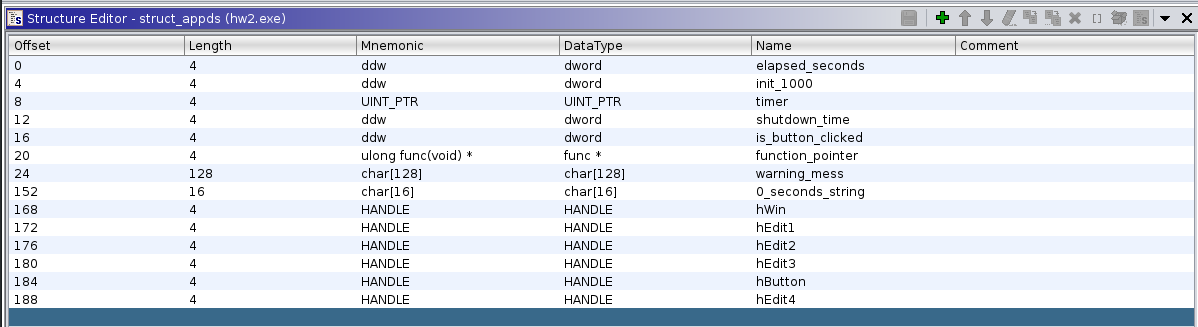
\includegraphics[width=\textwidth]{struct_appds_completa}
\end{figure}



\target{FUN_00401cf4_compute_shutdown_time}
\paragraph{FUN\_00401cf4\_compute\_shutdown\_time}
Questa funzione raccoglie i valori nelle caselle di testo e converte il valore dell'utente in minuti; esegue la seguente operazione:
\[
	m = days \cdot 1440 + hours \cdot 60 + minutes
\]
dove \emph{days, hours e minutes} sono i valori recuperati rispettivamente dalle caselle di giorni, ore e minuti. \\
Il valore $m$ così ottenuto, è utilizzato nel seguente calcolo:
\[
	\frac{m \cdot init\_1000 \cdot 60}{1000} + elapsed\_seconds
\]

Il risultato di questa operazione è il valore in secondi dopo il quale si vuole che il pc venga spento, e infatti viene memorizzato nel campo \code{shutdown_time} della struttura dati \code{struct_appds}. 

\newpage
\target{Verifica}
\section{Verifica}
Dopo aver inserito la password \textbf{3RnESt0!?} e dopo aver atteso il tempo selezionato, la macchina virtuale viene effettivamente spenta: il codice ottenuto dall'analisi è effettivamente il codice corretto.
 

\end{document}